\documentclass[9pt]{beamer}
\usepackage{minted}
%\usemintedstyle{manni}
\usemintedstyle{murphy}
\usepackage{hyperref}
\hypersetup{
colorlinks=true,
urlcolor=blue
}
\usepackage{graphicx}

\begin{document}
\title{Securing a Django (Wait, any!) Website}
\author{Nick Thompson} 
\date{\today}

\frame{\titlepage}

\begin{frame}[fragile]
\frametitle{Goals:}

\begin{itemize}
\item The information provided here should allow you to pass a rigorous security audit for cloud services, assuming your server has not been compromised.
\pause
\item This will not provide information about securing your server, only information about keeping data secure when it is on the wire.
\pause
\item More information about securing your server can be found \href{https://www.thefanclub.co.za/how-to/how-secure-ubuntu-1204-lts-server-part-1-basics}{elsewhere}.
\pause
\item Securing the wire is the easy part; harder is keeping authenticated users from grabbing other users data \emph{because that's code you write yourself}.
\end{itemize}
\end{frame}


\begin{frame}[fragile]
\frametitle{Getting started:}
\begin{minted}{bash}
$ git clone https://github.com/NAThompson/django_https.git
$ pyvenv django_https
$ cd django_https
$ pip3 install -r requirements.txt
$ sudo /bin/bash
$$ . bin/activate
\end{minted}
\pause
We'll need root to open up priviledged ports. Sourcing after acquisition of root shell is necessary.
\end{frame}

\begin{frame}
\frametitle{Server Stack}
\begin{itemize}
\item We're going to use Django+gunicorn+nginx to serve this website
\pause
\item \href{http://gunicorn.org/\#deployment}{gunicorn} is a web server gateway interface
\pause
\item We need nginx to reverse proxy because gunicorn is trivially vunerable to DOS attacks
\pause
\end{itemize}
\end{frame}

\begin{frame}[fragile]
\frametitle{Configuring Secure Settings}
\begin{itemize}
\item Many security settings can be configured either through nginx or through django-secure.
\pause
\item In my experience, nginx seems to be faster, so we'll focus on configuring nginx.
\pause 
\item django-secure settings will tend to override nginx settings, or they will be set twice in the http headers. So use nginx, or use django-secure, not both.
\end{itemize}
\end{frame}

\begin{frame}[fragile]
\frametitle{Configuring django-secure}
\begin{itemize}
\item Add the following to your INSTALLED\_APPS in settings.py:
\begin{minted}{python}
INSTALLED_APPS = (
    'sslserver',
    ...,
    'djangosecure',
)
\end{minted}
\pause
\item Then run the test server via:
\begin{minted}{bash}
$ ./manage.py checksecure 
$ ./manage.py runsslserver --addrport 127.0.0.1:443
\end{minted}
This is nice for development because it uses self-signed certificates with relative paths.
\end{itemize}
\end{frame}

\begin{frame}[fragile]
\frametitle{Install nginx}
\begin{minted}{bash}
$ sudo apt-get install nginx # Ubuntu
$ sudo brew install nginx # Mac
\end{minted}
\end{frame}

\begin{frame}[fragile]
\frametitle{Turn SSL on and proxy-pass to gunicorn}
\begin{minted}{bash}
server {
  listen         443;
  ssl            on;
  server_name    example.com;
  ssl_certificate  /somedir/bundle.crt;
  ssl_certificate_key /somedir/mykey.key;

  location / {
     proxy_pass https://127.0.0.1:8000;
     proxy_set_header Host $host;
     proxy_set_header X-Forwarded-For $proxy_add_x_forwarded_for;
  }
}
\end{minted}
\end{frame}

\begin{frame}[fragile]
\frametitle{How to serve the website}
\begin{minted}{bash}
$$ cd django_https/src
$$ gunicorn -c gunicorn_config.py https.wsgi &
$$ nginx -c ~/django_https/nginx.conf
\end{minted}
(Again, there are some hard-coded paths in this . . .)
\end{frame}

\begin{frame}[fragile]
\frametitle{How secure is the default nginx configuration?}
\begin{itemize}
\item \href{https://www.ssllabs.com/ssltest/analyze.html}{SSL Labs} doesn't think it's all that great:

\begin{figure}
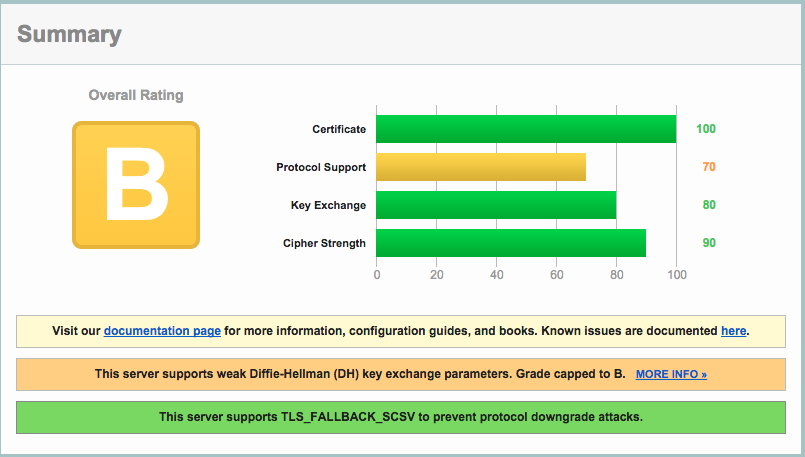
\includegraphics[scale=0.25]{figures/SSLLabsFirstGrade.png}
\end{figure}
\pause
\item If your clients have an IT policy, they \emph{will ask about this}.
\end{itemize}
\end{frame}

\begin{frame}[fragile]
\frametitle{Improving SSLLabs grade}
\begin{itemize}
\item In the nginx.conf, change 
\begin{minted}{c}
    ssl_protocols TLSv1 TLSv1.1 TLSv1.2;
\end{minted}
to
\begin{minted}{c}
    ssl_protocols TLSv1.2;
\end{minted}
\pause
\item Note: This will lose you some old IE browsers. SSLLabs will tell you which ones in the handshake simulation section of their report.
\end{itemize}
\end{frame}

\begin{frame}[fragile]
\frametitle{Some justification for only supporting TLSv1.2}
\begin{itemize}
\item The \href{https://www.pcisecuritystandards.org/}{Payment Card Industry (PCI) Security Standards Council} says you must remove support for TLSv1.0 to be PCI compliant. ``SSL and early TLS are not considered strong cryptography and cannot be used as a security control after 30th June, 2016.``
\pause
\item \href{https://www.owasp.org/index.php/Transport_Layer_Protection_Cheat_Sheet}{OWASP} (Open Web Application Security Project) claims ``TLS 1.0 is still widely used as 'best' protocol by a lot of browsers, that are not patched to the very latest version.  . . TLSv1.0 should only be used only after risk analysis and acceptance.``
\pause
\item Almost \href{https://en.wikipedia.org/wiki/Transport_Layer_Security\#Web_browsers}{no browsers} support TLSv1.1 and \emph{not} TLSv1.2. So make your life easier and just use 1.2.
\end{itemize}
\end{frame}

\begin{frame}[fragile]
\frametitle{Improving SSLLabs grade}
\begin{itemize}
\item SSLLabs thinks that 256 bits symmetric protocols are better than 128 bit protocols, although \href{https://www.schneier.com/blog/archives/2009/07/another_new_aes.html}{not everyone} agrees.
\pause 
\item But you can still improve your grade by restricting the supported ciphersuite by adding this to the http section of nginx.conf:
\begin{minted}{c}
ssl_ciphers ECDHE-RSA-AES256-GCM-SHA384:ECDHE-ECDSA-AES256-GCM-SHA384:ECDHE-RSA\
-AES256-SHA384:ECDHE-ECDSA-AES256-SHA384:ECDHE-RSA-AES256-SHA:ECDHE-ECDSA-AES256-SHA:DHE\
-RSA-AES256-GCM-SHA384:DHE-RSA-AES256-GCM-SHA:DHE-RSA-AES256-SHA256:DHE-RSA-AES256-SHA:!\
aNULL:!eNULL:!LOW:!3DES:!MD5:!EXP:!PSK:!SRP:!DSS;
\end{minted}
\pause
\item This is a mess, what does it mean?
\end{itemize}
\end{frame}

\begin{frame}
\frametitle{This configures \emph{ciphersuite negotiation}}
\begin{itemize}
\item The browser tells the server what ciphersuites it supports
\pause
\item The server selects one that is in the ssl\_ciphers list,
\pause
\item The server tells the browser what ciphers they are using, or rejects the connection if they can't agree on a cipher suite.
\end{itemize}
\end{frame}

\begin{frame}[fragile]
\frametitle{What is a ciphersuite?}
\pause
\begin{itemize}
\item A key exchange algorithm (generally an asymmetric cipher, e.g. RSA, Diffie-Hellman)
\pause
\item An bulk encryption algorithm (generally a symmetric cipher, e.g. AES)
\pause
\item A message authentication code algorithm  (hash function, SHA256)
\pause
\item An authentication protocol (e.g., RSA)
\end{itemize}
\end{frame}

\begin{frame}[fragile]
\frametitle{Understanding available ciphersuites}
To see what ciphers your nginx supports, run
\begin{minted}{bash}
$ openssl ciphers | tr ':' '\n'
\end{minted}
(nginx links against openssl's libraries)
\end{frame}

\begin{frame}[fragile]
\frametitle{Understanding available ciphersuites}
\begin{itemize}
\item To understand a given cipher, we use
\begin{minted}{bash}
$ openssl ciphers -v ECDHE-RSA-AES256-GCM-SHA384
ECDHE-RSA-AES256-GCM-SHA384
TLSv1.2 Kx=ECDH     Au=RSA  Enc=AESGCM(256) Mac=AEAD
\end{minted}
\pause
\item Kx = Key exchange; ECDH=elliptic curve Diffie-Hellman
\pause
\item Au=Authentication; uses RSA 
\pause
\item  Enc= Encryption; AESGCM(256) is 256 bit Advanced Encryption Standard in Galois Counter mode for encryption (please don't ask about GCM!)
\pause
\item Mac= Message Authentication; AEAD =``authentication encryption with associated data'' for message authentication (inherited from the ``Galois counter mode'' of AES)
\end{itemize}
\end{frame}


\begin{frame}[fragile]
\frametitle{Interpreting ssl\_ciphers}
Suppose this was our configuration:
\begin{minted}{c}
ssl_ciphers ECDHE-RSA-AES256-GCM-SHA384:ECDHE-ECDSA-AES256-GCM-SHA384;
\end{minted}
\begin{itemize}
\item The order matters: Adding ``ssl\_prefer\_server\_ciphers on;`` to the nginx.conf tells nginx to ignore the preferences of the browser.
\pause
\item So first we would use ECDHE-RSA-AES256-GCM-SHA384, but if the browser doesn't support it, then we use ECDHE-ECDSA-AES256-GCM-SHA384.
\pause
\item Otherwise, we don't make the connection to the browser.
\end{itemize}
\end{frame}


\begin{frame}
\frametitle{What ciphersuites does my browser support?}
There are \href{https://cc.dcsec.uni-hannover.de/}{some websites} who will tell you:
\begin{figure}
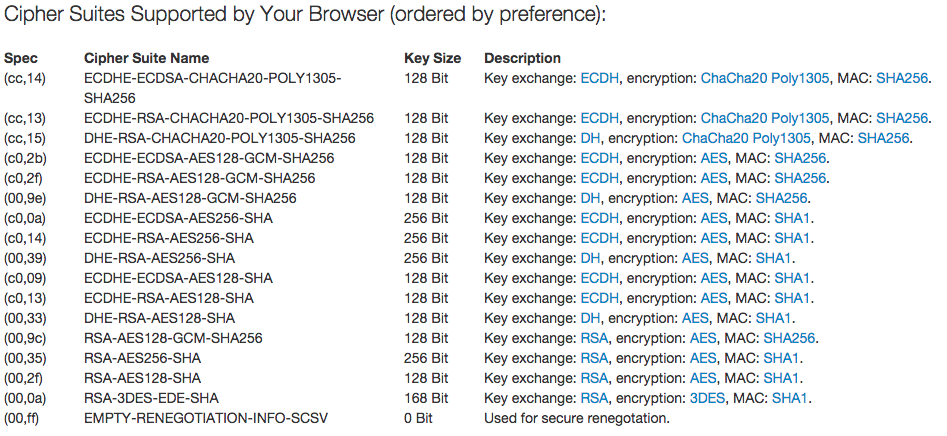
\includegraphics[scale=0.25]{figures/browserciphersuites.png}
\end{figure}
\end{frame}

\begin{frame}[fragile]
\frametitle{Some advice:}
\begin{itemize}
\item Prefer Galois counter modes (AES-GCM) as they consume less resources
\pause
\item Prefer SHA256 over SHA1 as SHA1 will be \href{http://googleonlinesecurity.blogspot.com/2014/09/gradually-sunsetting-sha-1.html}{deprecated}.
\pause
\item Make sure to sign your certificates with SHA256 over SHA1, or else it will not be trusted by Google Chrome.
\pause
\item \href{https://www.nsa.gov/business/programs/elliptic_curve.shtml}{Prefer} elliptic curves, unless you think the NSA has a \href{https://en.wikipedia.org/wiki/Elliptic_curve_cryptography}{quantum computer}.
\end{itemize}
\end{frame}

\begin{frame}[fragile]
\frametitle{Defense Against the Logjam attack}
\begin{itemize}
\item The \href{https://weakdh.org/}{logjam} attack was discovered relatively recently, and is an attack against Diffie-Hellman key exchange. 
\pause
\item It's thought that it was only used by state-level adversaries, but it seems that this will change soon.
\end{itemize}
\end{frame}

\begin{frame}[fragile]
\frametitle{Diffie-Hellman Key Exchange Review}
\begin{itemize}
\item Server picks a prime $p$ and $g < p$ along with random $a< p$. $p$ and $g$ are public, $a$ is secret. 
\pause
\item Over the network is transferred $A := g^{a} \mod p$, $g$, $p$, cryptographically signed.
\pause
\item Client chooses $b < p$ and sends the server $B = g^{b}\mod p$.
\pause
\item The shared secret is $s := g^{ab} \mod p$.
\pause
\end{itemize}
This is a secure protocol as solving $A = g^{a} \mod p$ for $a$ (called ``the discrete logarithm'') is hard.
\end{frame}

\begin{frame}[fragile]
\frametitle{Diversion: Enabling Forward Secrecy}
 ``. . . which \href{https://www.owasp.org/index.php/Transport_Layer_Protection_Cheat_Sheet}{means} a compromise of the server's long term signing key does not compromise the confidentiality of past session'' 
\end{frame}

\begin{frame}[fragile]
\frametitle{Diversion: Forward secrecy in Diffie-Hellman}
\begin{itemize}
\item Question: What does the server do with $a$ (the random secret) after the SSL session ends?
\pause
\item  Can the NSA subpoena your Diffie-Helman session keys?
\end{itemize}
\end{frame}

\begin{frame}[fragile]
\frametitle{What if it takes 2 minutes to generate a prime $p$ for Diffie-Hellman key exchange?}
\begin{itemize}
\item Then everyone uses the same damn prime.
\pause
\item ``\href{http://blog.cryptographyengineering.com/2015/05/attack-of-week-logjam.html}{The} situation for export Diffie-Hellman is particularly awful, with only two (!) primes used across up 92\% of enabled Apache/mod\_ssl sites.''
\end{itemize}
\end{frame}

\begin{frame}[fragile]
\frametitle{What if we have to support 20 year old browsers?}
\begin{itemize}
\item Then an attacker can do a downgrade attack so that the prime $p$ is only 512 bits.
\pause
\item This allows a MITM to intercept your server message, and send it saying ``we only support 512 bit DH''; the browser supports it, so it agrees to use of export-grade crypto.
\end{itemize}
\end{frame}

\begin{frame}[fragile]
\frametitle{What if the prime $p$ is only 512 bits? That's still a lot}
\begin{itemize}
\item Solving a 512 bit discrete logarithm is hard; it takes an academic group about a week.
\pause
\item But for fixed $p$, using a \emph{very sophisticated} lookup table, computing the \emph{next} discrete log only takes 90 seconds.
\pause
\end{itemize}
The \href{https://weakdh.org/sysadmin.html}{solution} is . . .
\end{frame}

\begin{frame}[fragile]
\frametitle{Generating a large, unique Diffie-Hellman Prime}
\begin{minted}{bash}
$ openssl dhparam -out dhparam.pem 4096
\end{minted}
and add the following line to the nginx.conf:
\begin{minted}{bash}
ssl_dhparam /path_to_pem/dhparam.pem
\end{minted}
\end{frame}

\begin{frame}[fragile]
\frametitle{SSLLabs is now Happy}
\begin{figure}
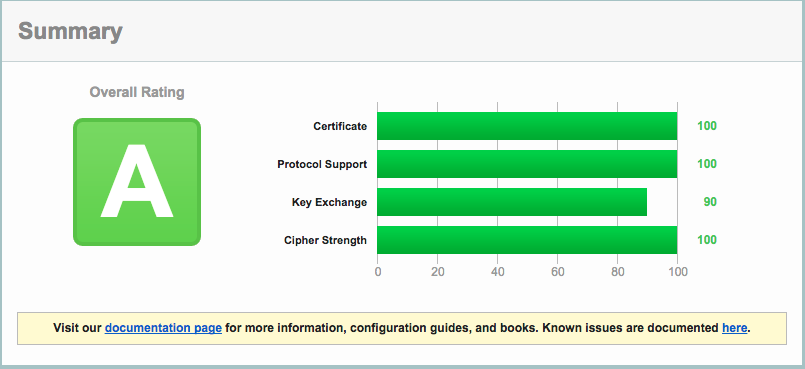
\includegraphics[scale=0.25]{figures/SSLLabsA.png}
\end{figure}
You can see the SSLLabs rating guide \href{https://www.ssllabs.com/downloads/SSL_Server_Rating_Guide.pdf}{here}.
\end{frame}

\begin{frame}[fragile]
\frametitle{What is HTTP Strict Transport Security? (HSTS)}
\begin{itemize}
\item A protocol by which servers force all traffic to come over https.
\pause
\item Server informs browser to recognize MITM attack by requests for http traffic
\pause
\item Stops downgrade attacks and cookie hijacking.
\pause
\item Stops \href{http://www.thoughtcrime.org/software/sslstrip/}{SSL stripping!}
\end{itemize}
\end{frame}

\begin{frame}[fragile]
\frametitle{HSTS}
A user who has visited your site previously \emph{cannot} proceed past a bad certificate:
\begin{figure}
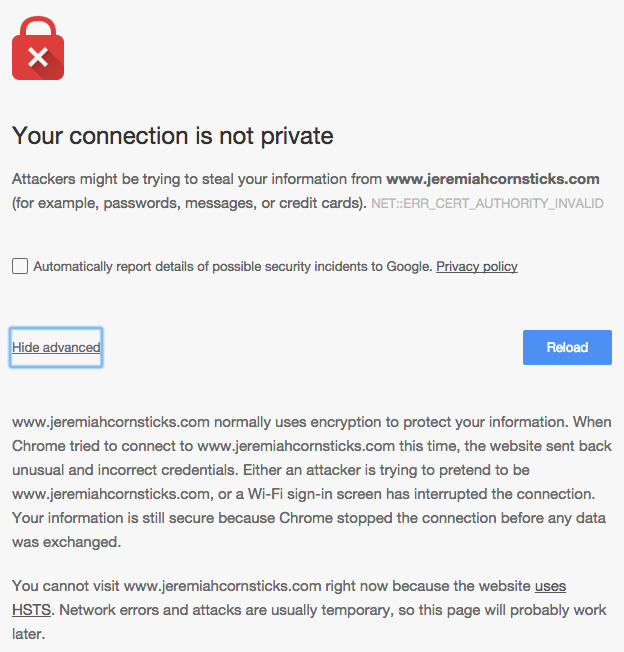
\includegraphics[scale=0.25]{figures/HSTSNoRedirect.png}
\end{figure}
\pause
(Unless they clear their browser cache . . . then the user can ignore the warning and proceed.)
\end{frame}

\begin{frame}[fragile]
\frametitle{HSTS Redirects http to https}
\emph{But only after a user visits the first time . . .}
\pause
\begin{itemize}
\item Workaround for first-time users:
\pause
\item Register your site in the \href{https://hstspreload.appspot.com/}{preload list!}
\pause
\item ``This form is used to submit domains for inclusion in Chrome's HTTP Strict Transport Security (HSTS) preload list. This is a list of sites that are hardcoded into Chrome as being HTTPS only.''
\end{itemize}
\end{frame}

\begin{frame}[fragile]
\frametitle{Configuring HSTS}
\begin{itemize}
\item Add this to the server section in ``default'':
\begin{minted}{c}
add_header Strict-Transport-Security \
 "max-age=63072000; includeSubdomains";
\end{minted}
\begin{figure}
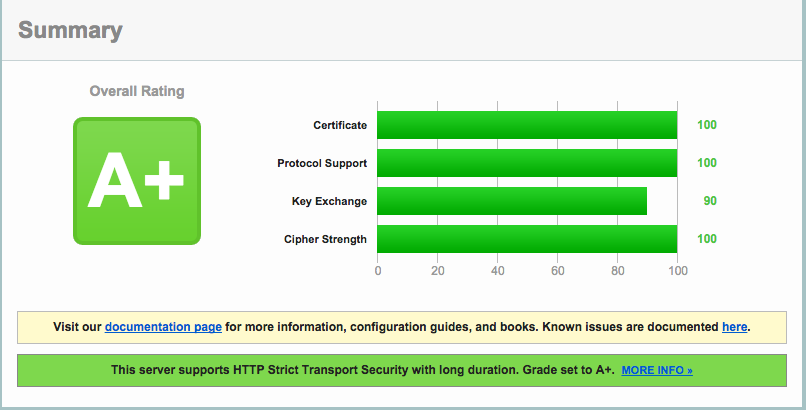
\includegraphics[scale=0.25]{figures/SSLLabsAp.png}
\end{figure}
\pause
\item The server now says: ``For the next 63072000 seconds, this server and its subdomains will only be using https. Any http traffic is a MITM attack.''
\end{itemize}
\end{frame}

\begin{frame}[fragile]
\frametitle{HSTS Configured in django-secure}
\begin{itemize}
\item Add the following to your settings.py:
\begin{minted}{python}
SECURE_HSTS_SECONDS = 63072000
SECURE_HSTS_SUBDOMAINS = True
SECURE_HSTS_INCLUDE_SUBDOMAINS = True
\end{minted}
\pause
\item Not that this will override the nginx settings, if you set them both.
\end{itemize}
\end{frame}

\begin{frame}[fragile]
\frametitle{Debugging Aid:}
\begin{itemize}
\item The server's use of HSTS is communicated via http headers, and nginx doesn't do a strong validation of the nginx.conf. In addition, nginx version changes can silently break your nginx.conf.
\pause
\item To validate that you've actually set a http header:
\pause
\item Use ``Live HTTP Headers'' Chrome browser extension (I like it!)
\pause 
\item Use alt-command-I on Chrome (more painful)
\pause 
\item Use Wireshark
\end{itemize}
\end{frame}

\begin{frame}[fragile]
\frametitle{Debugging http headers:}
Example using Live HTTP headers Chrome extension:
\begin{figure}
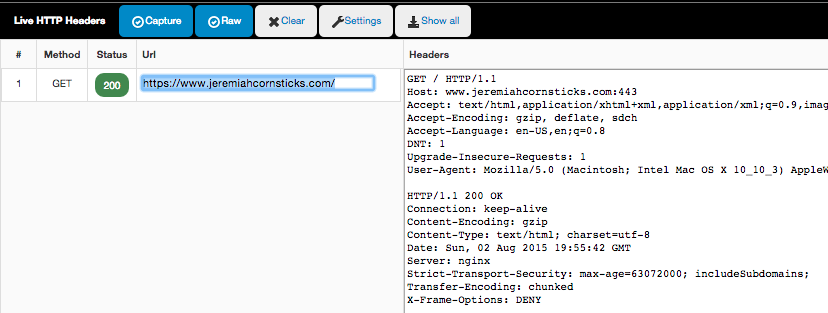
\includegraphics[scale=0.35]{./figures/xframedeny.png}
\end{figure}
\end{frame}


\begin{frame}[fragile]
\frametitle{Strong key-exchange}
To get a strong key-exchange, we need at least 4096 bit keys:
\pause
\begin{minted}{bash}
$ openssl genrsa -out foo.key 4096; chmod 400 foo.key;
$ openssl req -new -sha256 -key foo.key -out foo.csr
\end{minted}
\pause
Use this certificate signing request to get certs from your provider, and you're done!
\begin{figure}
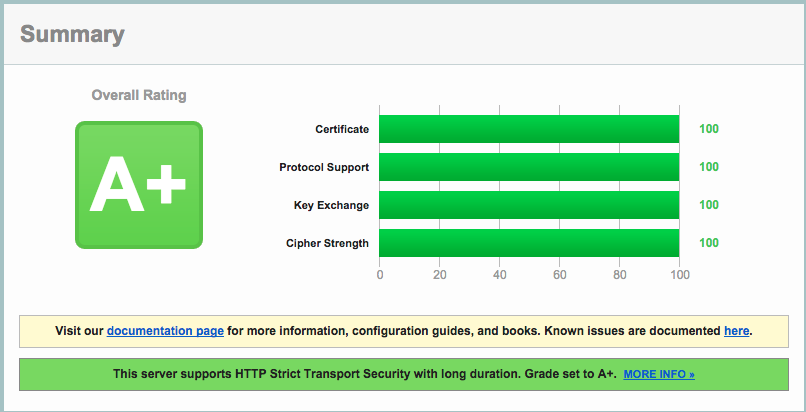
\includegraphics[scale=0.25]{figures/App.png}
\end{figure}
\end{frame}

\begin{frame}[fragile]
\frametitle{OCSP Stapling}
\begin{itemize}
\item OCSP := Online Certificate Status Protocol
\pause
\item Used to determine if a certificate has been revoked
\pause
\item Browsers must query certificate authority (CA), revealing websites they visit
\pause
\item OCSP Stapling: Server caches CA's OCSP digitally signed response, increasing privacy as well as speed
\end{itemize}
\end{frame}

\begin{frame}[fragile]
\frametitle{Enabling OCSP Stapling in nginx}
\begin{itemize}
\item Bundle intermediate and root certifications:
\begin{minted}{bash}
cat  foo1.crt foo2.crt > ocsp.crt;
\end{minted}
Since I bought \$5 certificates for this talk, I did:
\begin{minted}{bash}
 cat COMODORSADomainValidationSecureServerCA.crt \
  COMODORSAAddTrustCA.crt > ocsp.crt
\end{minted}
\pause
\item Then add the following lines to the nginx.conf:
\begin{minted}{c}
  resolver 8.8.8.8;
  ssl_stapling on;
  ssl_stapling_verify on;
  ssl_trusted_certificate /pathtocerts/ocsp.crt;
\end{minted}
\end{itemize}
\end{frame}

\begin{frame}[fragile]
\frametitle{Diversion: Certificate Authorities}
\begin{itemize}
\item Free, trusted certificates coming next month from \href{https://letsencrypt.org/}{Let's Encrypt}
\end{itemize}
\end{frame}

\begin{frame}[fragile]
\frametitle{Clickjacking}
\begin{itemize}
\item Someone renders your page in theirs (example: ebay.com/buynicecar)
\pause
\item Then they make your page invisible, but put ``Win free iPad!'', and a place to click over the ``Buy it now'' link of the ebay listing
\pause
\item If you are logged in on ebay, you are the proud owner of a new car!
\end{itemize}
\end{frame}

\begin{frame}[fragile]
\frametitle{Clickjacking}
``\href{https://www.owasp.org/index.php/Clickjacking}{One} of the most notorious examples of Clickjacking was an attack against the Adobe Flash plugin settings page. By loading this page into an invisible iframe, an attacker could trick a user into altering the security settings of Flash, giving permission for any Flash animation to utilize the computer's microphone and camera.''
\end{frame}

\begin{frame}[fragile]
\frametitle{Defense against clickjacking}
As a web user: You're screwed.
\end{frame}

\begin{frame}[fragile]
\frametitle{Defense against clickjacking}
\begin{itemize}
\item As a developer: Add the following to your nginx.conf:
\begin{minted}{c}
add_header X-Frame-Options DENY;
\end{minted}
\pause
\item Or to your settings.py:
\begin{minted}{python}
SECURE_FRAME_DENY = True
\end{minted}
\pause
\item Note that this is a non-standard extension to html. There is a standardized way (see content security policies), but it's not yet supported by all modern browsers
\end{itemize}
\end{frame}

\begin{frame}[fragile]
\frametitle{Defense against clickjacking}
\begin{itemize}
\item This is such a huge problem that the default django configuration actually sets the http response header ``X-Frame-Options: SAMEORIGIN'':
\begin{minted}{python}
MIDDLEWARE_CLASSES = (
...
'django.middleware.clickjacking.XFrameOptionsMiddleware',
...
)
\end{minted}
\pause
\item SAMEORIGIN means you can embed your own webpages in html frames, but disallows its embedding in other people's websites.
\end{itemize}
\end{frame}

\begin{frame}
\frametitle{Verify the http header}
Again, verify that the \texttt{X-Frame-Options: DENY} header has been sent:
\begin{figure}
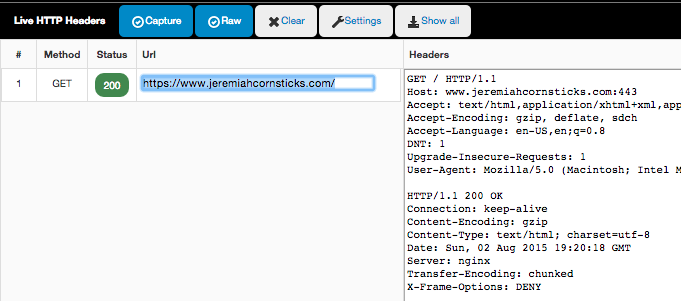
\includegraphics[scale=0.35]{./figures/debugging_http_headers.png}
\end{figure}
\end{frame}

\begin{frame}[fragile]
\frametitle{Content Sniffing}
\begin{itemize}
\item Some html content is not given the proper tags for its interpretation
\pause
\item So Microsoft decided to give IE the capacity to guess the interpretation of a byte-stream, called content-sniffing
\pause
\item And that algorithm sucks.
\end{itemize}
\end{frame}

\begin{frame}[fragile]
\frametitle{Content Sniffing}
\begin{itemize}
\item By using bugs in the IE content sniffer, users can be deceived about what sort of content they are downloading (they thing .jpg, they get a script).
\pause
\item This is mainly a problem on sites where users can both upload and download data.
\end{itemize}
\end{frame}

\begin{frame}[fragile]
\frametitle{Preventing Content Sniffing Attacks}
\begin{itemize}
\item Add the following to the nginx.conf:
\begin{minted}{c}
add_header X-Content-Type-Options nosniff;
\end{minted}
\pause
\item Or to your settings.py:
\begin{minted}{python}
SECURE_CONTENT_TYPE_NOSNIFF = True
\end{minted}
\end{itemize}
\end{frame}

\begin{frame}[fragile]
\frametitle{Diminishing Returns}
\begin{itemize}
\item nginx announces its version to all the world
\pause
\item This makes life easy for zero-day hoarders
\pause
\item Make life \emph{a bit} harder for them by adding this to the http section of nginx.conf:
\begin{minted}{c}
server_tokens off;
\end{minted}
\pause
\item SSLlabs can still determine that nginx is serving the website, but doesn't know the version.
\end{itemize}
\end{frame}

\end{document}
